%%%%%%%%%%%%%%%%%%%%%%%%%%%%%%%%%%%%%%%%%
% Diaz Essay
% LaTeX Template
% Version 2.0 (13/1/19)
%
% This template originates from:
% http://www.LaTeXTemplates.com
%
% Authors:
% Vel (vel@LaTeXTemplates.com)
% Nicolas Diaz (nsdiaz@uc.cl)
%
% License:
% CC BY-NC-SA 3.0 (http://creativecommons.org/licenses/by-nc-sa/3.0/)
%
%%%%%%%%%%%%%%%%%%%%%%%%%%%%%%%%%%%%%%%%%

%----------------------------------------------------------------------------------------
%	PACKAGES AND OTHER DOCUMENT CONFIGURATIONS
%----------------------------------------------------------------------------------------

\documentclass[12pt]{diazessay} % Font size (can be 10pt, 11pt or 12pt)
% \languagepath{brazil}
% \deftranslation[to=brazil]{Example}{Exemplo}
% \deftranslation[to=brazil]{Theorem}{Teorema}

%----------------------------------------------------------------------------------------
%	TITLE SECTION
%----------------------------------------------------------------------------------------

\title{\textbf{Identificação de Locutor} \\ {\Large\itshape Utilizando MFC e GMMs}} % Title and subtitle

\author{\textbf{Ramon Duarte de Melo \\ André Ribeiro Queiroz} \\ \textit{Universidade Federal do Rio de Janeiro}} % Author and institution

\date{\today} % Date, use \date{} for no date

%----------------------------------------------------------------------------------------

\begin{document}

\maketitle % Print the title section

%----------------------------------------------------------------------------------------
%	ABSTRACT AND KEYWORDS
%----------------------------------------------------------------------------------------

%\renewcommand{\abstractname}{Summary} % Uncomment to change the name of the abstract to something else

\begin{abstract}
	Realizamos uma implementação de identificação de locutor utilizando a técnica de \emph{Mel-frequency cepstrum} (MFC) para a extração das informações e modelos misturados de gaussianas (GMM) para os classificadores.
	Foram realizadas variações de duração da janela, afastamento entre janelas subsequentes (offset), quantidade de coeficientes de MFC e função de janelamento.
	O sistema foi implementado com base na biblioteca \texttt{python\_speech\_features} e nos módulos de métodos numéricos \texttt{scipy} e \texttt{numpy}.
	Observamos que o \emph{offset} é o maior preditor de melhora da taxa de sucesso, produzindo resultados melhores quanto menor o afastamento (e maior a sobreposição).
	O número de coeficientes também foi significativo, com os melhores resultados sendo observados para as baterias de testes que envolviam 20 MFCCs.
	A duração da janela e a função de janelamento afetaram pouco as taxas de sucesso neste trabalho.

\end{abstract}

\hspace*{3.6mm}\textit{Palavras-chave:} \emph{Mel-frequency cepstrum}, modelos misturados de gaussianas, identificação de locutor % Keywords

\vspace{10pt} % Vertical whitespace between the abstract and first section

%----------------------------------------------------------------------------------------
%	ESSAY BODY
%----------------------------------------------------------------------------------------

\section*{Introdução}

A motivação inicial para este trabalho é a aplicação de identificação de locutor em cenários onde desempenho crítico não é exigido.
Por exemplo, podemos imaginar um software de conferência que conecte usuários com níveis distintos de hierarquia ou privilégios.
Quando um usuário com alto privilégio (por exemplo, o CEO de uma companhia) falar, o software poderá identificá-lo como de alto privilégio e proceder com o silenciamento dos microfones dos demais usuários, evitando interrupções ou conversas convolutas.

O sistema foi construído com a biblioteca \texttt{python\_speech\_features}, que fornece o método \texttt{mfcc()} para a extração dos coeficientes de \emph{Mel-frequency cepstrum}, bem como de seus diferenciais (ou deltas, ou coeficientes dinâmicos).
Em seguida, os classificadores foram construídos com o método \texttt{scipy.gmm()}, que permite a gravação dos modelos sob arquivos \texttt{.gmm} que podem ser manipulados de forma ágil no momento de testes.
Para o armazenamento persistente das informações, foram utilizados arquivos de texto plano, por não serem dados sensíveis e por serem fáceis de serem armazenados em repositórios de sistemas de versionamento como o \texttt{git}.

Os resultados foram analisados num \texttt{jupyter-notebook} através de tabelas de dados (\emph{dataframes}) do \texttt{pandas} e métodos numéricos do \texttt{numpy}.
Os gráficos foram produzidos pela biblioteca \texttt{matplotlib.pyplot}.
Ao longo de todo o trabalho, a linguagem utilizada foi \emph{Python 3.6.7}.

%------------------------------------------------

\section*{Implementação}

O seguinte pipeline foi construído para o sistema:

\begin{enumerate}
	\item Dados dos locutores alimentam o treinamento dos modelos.
	\item Os sinais são amostrados e janelados durante o pré-processamento.
	\item Os coeficientes e seus deltas são extraídos do dataset de treino.
	\item Modelos misturados de gaussianas são utilizados para a modelagem estatística, de forma a tentar predizer a distribuição de MFCCs.
	\item Os GMMs são gravados em disco para quando forem necessários ao teste.
	\item Dados dos locutores para serem adivinhados alimentam o sistema pela interface de testes.
	\item Os classificadores (GMMs treinados) são carregados do disco para produzirem probabilidades de cada locutor.
	\item O sistema opta pelo locutor com maior probabilidade e retorna sua identificação.
	\item Uma nota $1$ é atribuída ao resultado caso o locutor retornado seja o mesmo do locutor testado; caso contrário, é atribuída a nota $0$. 
\end{enumerate}

\begin{figure}
	\centering
	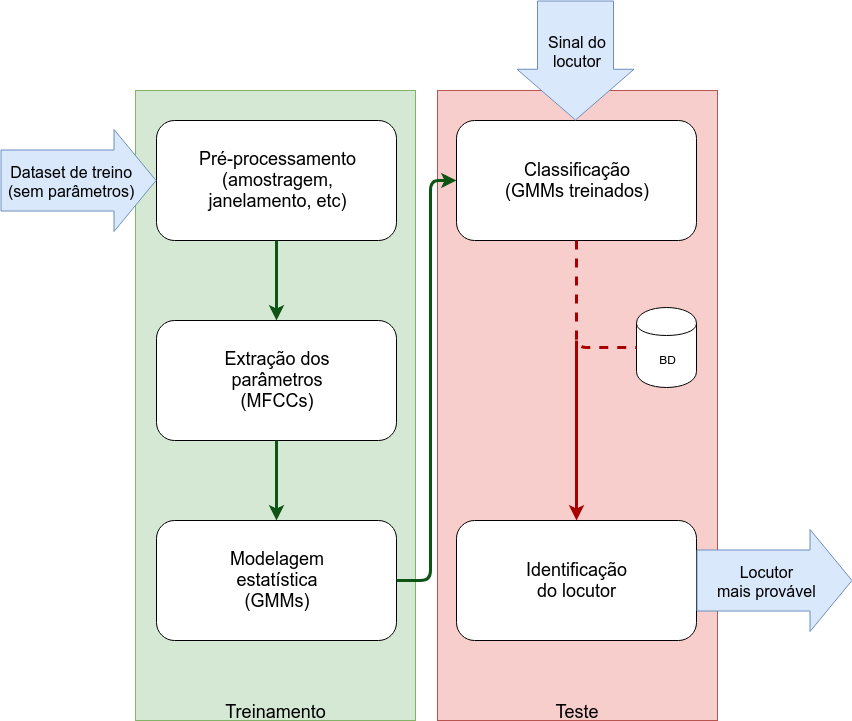
\includegraphics[width=\linewidth]{fig2.png}
	\caption{Arquitetura do sistema de identificação de locutor.}
\end{figure}

O dataset utilizado possui 34 locutores com 10 observações cada e foram adquiridos do fórum \emph{VoxForge.com}.
Os áudios foram disponibilizados sob a licença \emph{Creative Commons} e, portanto, podem ser utilizados livremente, desde que a fonte seja mencionada.

Metade do dataset foi utilizado para o treinamento, especificamente as 5 observações mais longas de cada locutor.
A maioria esmagadora dos áudios possuem entre 20 e 30 segundos.
No entanto, há áudios que se aproximam dos 60 segundos.

Em todo caso, este dataset possui áudios incomumente longos, visto que a maioria dos sistemas de identificação de locutor trabalham com poucos segundos.
A outra metade foi utilizada para os testes, tendo a maioria deles sido feitos com áudios de cerca de 10 segundos.
Os áudios estão todos amostrados em 16 kHz, com 16 bits por amostra.

Os parâmetros variáveis no sistema são:

\begin{enumerate}
	\item Número de coeficientes: qualquer número de MFCCs estáticos pode ser inserido como entrada. Entretanto, o número de coeficientes dinâmicos será obrigatoriamente igual ao de estáticos. Somente os primeiros diferenciais podem ser utilizados. Para este trabalho, foram utilizados $12 + 12$, $16 + 16$, $20 + 20$ e $24 + 24$ coeficientes.
	\item Duração da janela: foram utilizados valores típicos para este parâmetro: 20, 25 e 30 ms.
	\item Afastamento entre janelas (\emph{offset}): o valor mais comumente utilizado na literatura é de 5 ms, mas também foram testados 10, 15 e 20 ms.
	\item Função de janelamento: estes parâmetros são passados diretamente ao \texttt{scipy} (sem filtragem ou \emph{parsing}) e, portanto, todas as funções de janelamento oferecidas por sua API estão disponíveis, como Blackman, Poisson, cossenoide, gaussiana, Hamming, Hanning e triangular. Para este trabalho, foram consideradas as funções de Blackman e de Hamming.
\end{enumerate}

Os resultados obtidos foram analisados através da taxa de sucesso, do cálculo do desvio-padrão de suas distribuições, e de suas correlações lineares. 

%------------------------------------------------

\section*{Conclusão}

Os resultados obtidos exibiram, no geral, taxas de sucesso bastante elevadas, com nenhuma das combinações produzindo taxas de sucesso inferiores a 80\%.
Quatro combinações acertaram todas as 170 anotações e receberam a taxa de sucesso de 100\%.
A maioria das demais oscilou entre 90 e 100\% de acerto.

\begin{figure}
	\centering
	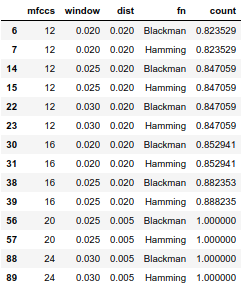
\includegraphics[width=0.55\linewidth]{Figure_6.png}
	\caption{Piores (10 primeiras linhas) e melhores (4 últimas linhas) combinações de acordo com a taxa de acerto da bateria de testes.}
\end{figure}

\begin{figure}
	\centering
	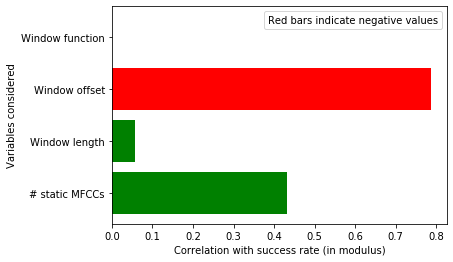
\includegraphics[width=0.85\linewidth]{Figure_5.png}
	\caption{Módulo da correlação linear dos parâmetros com a taxa de sucesso.}
\end{figure}

O parâmetro com maior impacto sobre a taxa de sucesso foi o afastamento entre uma janela e outra.
Sua correlação com a taxa de acerto, em módulo, foi a maior deste trabalho, indicando que a redução das sobreposições afeta muito negativamente a eficácia do sistema.

\begin{figure}
	\centering
	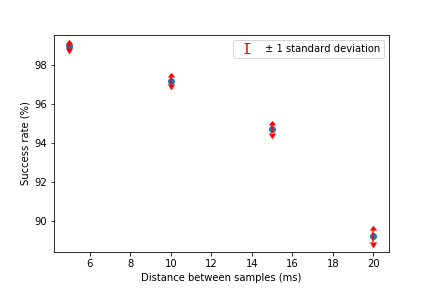
\includegraphics[width=0.85\linewidth]{Figure_3.png}
	\caption{Taxa de sucesso de acordo com o \emph{offset} da janela.}
\end{figure}

O impacto do número de coeficientes foi o mais significativo depois do \emph{offset}.
Porém, nesta distribuição é possível observar que o número ótimo de coeficientes aproxima-se de $20 + 20$, começando a cair quando este valor é superado.

\begin{figure}
	\centering
	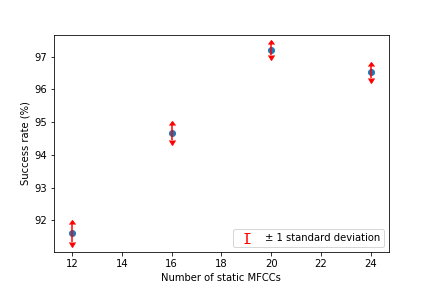
\includegraphics[width=0.85\linewidth]{Figure_1.png}
	\caption{Taxa de sucesso em função da quantidade de coeficientes estáticos utilizados.}
\end{figure}

A função de janelamento teve quase nenhum impacto sobre a taxa de acerto.
Observe que a correlação com a função de janelamento não é nula, mas desprezível, sendo da ordem de $10^{-15}$ ponto percentual.
Ao longo de mais de 16000 observações, houve apenas 4 divergências causadas pelas funções de Blackman e de Hamming.
A diferença entre ambas, invisível a olho nu, foi de $0,0245$ ponto percentual.

\begin{figure}
	\centering
	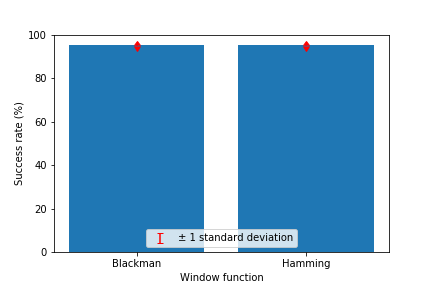
\includegraphics[width=0.65\linewidth]{Figure_4.png}
	\caption{Taxa de sucesso de acordo com a função de janelamento utilizada. }
\end{figure}


Similarmente, a duração da janela afetou muito pouco as predições.
Contudo, isto provavelmente se deve às janelas usadas aqui serem amplamente utilizadas na literatura. 
Com mais valores, a expectativa é de que haja maior correlação entre duração da janela e taxa de sucesso.

\begin{figure}
	\centering
	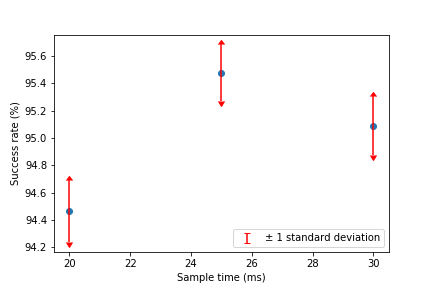
\includegraphics[width=0.65\linewidth]{Figure_2.png}
	\caption{Taxa de sucesso de acordo com a duração da janela.}
\end{figure}

%----------------------------------------------------------------------------------------

\end{document}
